\gdef\tagBrand{NT}
\gdef\footerAddress{Zalo: 0799666070}
\setcounter{ex}{0}
\setcounter{bt}{0}

% --- CÂU 1 ---
\begin{ex}
	Cho hai tập hợp $A = (-\infty; 3]$ và $B = (-2; 6)$.
	\begin{enumerate}[a)]
		\item Xác định các tập hợp $A \cup B$ và $A \cap B$.
		\item Giải thích việc lấy hoặc loại các điểm đầu mút trong các kết quả tìm được ở câu a.
	\end{enumerate}
	\loigiai{
		\begin{enumerate}[a)]
			\item Ta có:
			\begin{itemize}
				\item $A \cup B = (-\infty; 6)$.
				\item $A \cap B = (-2; 3]$.
			\end{itemize}
			\item Giải thích chi tiết việc lấy hoặc loại các điểm đầu mút:
			\begin{itemize}
				\item Đối với $A \cup B = (-\infty; 6)$:
				\begin{itemize}
					\item Đầu mút $-\infty$: Do tập hợp $A = (-\infty; 3]$ không bị chặn dưới nên hợp của hai tập hợp cũng không bị chặn dưới.
					\item Đầu mút $6$: Ta có $6 \notin B$ và $6 \notin A$, do đó $6 \notin (A \cup B)$. Vì vậy, tại đầu mút $6$ ta dùng ngoặc tròn loại điểm $6$.
				\end{itemize}
				\item Đối với $A \cap B = (-2; 3]$:
				\begin{itemize}
					\item Đầu mút $-2$: Ta thấy $-2 \in A$ nhưng $-2 \notin B$, nên $-2 \notin (A \cap B)$. Do đó tại đầu mút $-2$ ta dùng ngoặc tròn loại điểm $-2$.
					\item Đầu mút $3$: Điểm $3 \in A$ (do ngoặc vuông tại $3$) và $3 \in B$ (vì $-2 < 3 < 6$), nên $3 \in (A \cap B)$. Do đó tại đầu mút $3$ ta dùng ngoặc vuông lấy điểm $3$.
				\end{itemize}
			\end{itemize}
		\end{enumerate}
	}
\end{ex}

% --- CÂU 2 ---
\begin{ex}
	Cho bất phương trình bậc nhất hai ẩn $2x - y \le 4$.
	\begin{enumerate}[a)]
		\item Biểu diễn miền nghiệm của bất phương trình trên mặt phẳng tọa độ $Oxy$.
		\item Điểm $M(1; -3)$ có thuộc miền nghiệm của bất phương trình đã cho không? Giải thích.
	\end{enumerate}
	\loigiai{
		\begin{enumerate}[a)]
			\item Biểu diễn miền nghiệm:
			\begin{itemize}
				\item Vẽ đường thẳng $d\colon 2x - y = 4$. Đường thẳng $d$ đi qua hai điểm $(0; -4)$ và $(2; 0)$.
				\item Chọn điểm $O(0; 0)$ không thuộc đường thẳng $d$. Thay tọa độ $(0; 0)$ vào vế trái bất phương trình:
				$$2 \cdot 0 - 0 = 0 \le 4\text{ (mệnh đề đúng)}.$$
				\item Vậy miền nghiệm của bất phương trình là nửa mặt phẳng có bờ là đường thẳng $d$, chứa gốc tọa độ $O(0; 0)$ (kể cả bờ $d$).
			\end{itemize}
			\begin{center}
				\begin{tikzpicture}[>=stealth, scale=0.8, line join=round, line cap=round]
					% Trục tọa độ
					\draw[->,line width=0.8pt] (-2.5,0) -- (4.5,0) node[below] {$x$};
					\draw[->,line width=0.8pt] (0,-5) -- (0,2.5) node[left] {$y$};
					\node[below left] at (0,0) {$O$};
					
					% Các vạch chia
					\foreach \x in {-2,-1,1,2,3,4}
						\draw (\x,1pt) -- (\x,-1pt) node[below, font=\footnotesize] {$\x$};
					\foreach \y in {-4,-3,-2,-1,1,2}
						\draw (1pt,\y) -- (-1pt,\y) node[left, font=\footnotesize] {$\y$};
					
					% Miền không thỏa mãn (bị gạch)
					\fill[pattern=north east lines, pattern color=gray!60] (-0.5,-5) -- (4,-5) -- (4,4) -- (3,2) -- cycle;
					
					% Đường thẳng biên d: 2x - y = 4 => y = 2x - 4
					\draw[line width=1.2pt, blue!80!black] (-0.5,-5) -- (3.25,2.5) node[right] {$d\colon 2x - y = 4$};
					
					% Điểm đặc biệt
					\filldraw[black] (2,0) circle (1.5pt);
					\filldraw[black] (0,-4) circle (1.5pt);
				\end{tikzpicture}
			\end{center}
			\item Thay tọa độ $M(1; -3)$ vào vế trái của bất phương trình:
			$$2 \cdot 1 - (-3) = 2 + 3 = 5.$$
			Vì $5 > 4$ nên khẳng định $5 \le 4$ là sai.\\
			Vậy điểm $M(1; -3)$ không thuộc miền nghiệm của bất phương trình đã cho.
		\end{enumerate}
	}
\end{ex}

% --- CÂU 3 ---
\begin{ex}
	Cho góc $\alpha$ thỏa mãn $0^\circ < \alpha < 90^\circ$ và $\cos\alpha = \dfrac{4}{5}$.
	\begin{enumerate}[a)]
		\item Tính $\sin\alpha$ và $\tan\alpha$.
		\item Tính giá trị của biểu thức $P = \dfrac{2\sin\alpha + 3\cos\alpha}{4\sin\alpha - \cos\alpha}$.
	\end{enumerate}
	\loigiai{
		\begin{enumerate}[a)]
			\item Vì $0^\circ < \alpha < 90^\circ$ nên $\sin\alpha > 0$. Ta có:
			$$\sin\alpha = \sqrt{1 - \cos^2\alpha} = \sqrt{1 - \left(\dfrac{4}{5}\right)^2} = \sqrt{\dfrac{9}{25}} = \dfrac{3}{5}.$$
			Suy ra:
			$$\tan\alpha = \dfrac{\sin\alpha}{\cos\alpha} = \dfrac{\frac{3}{5}}{\frac{4}{5}} = \dfrac{3}{4}.$$
			\item Thay $\sin\alpha = \dfrac{3}{5}$ và $\cos\alpha = \dfrac{4}{5}$ vào biểu thức $P$, ta được:
			$$P = \dfrac{2 \cdot \dfrac{3}{5} + 3 \cdot \dfrac{4}{5}}{4 \cdot \dfrac{3}{5} - \dfrac{4}{5}} = \dfrac{\dfrac{6}{5} + \dfrac{12}{5}}{\dfrac{12}{5} - \dfrac{4}{5}} = \dfrac{\dfrac{18}{5}}{\dfrac{8}{5}} = \dfrac{18}{8} = \dfrac{9}{4}.$$
		\end{enumerate}
	}
\end{ex}

% --- CÂU 4 ---
\begin{ex}
	Một cơ sở sản xuất đồ lưu niệm may hai loại túi thủ công: loại túi nhỏ $A$ và loại túi lớn $B$.
	\begin{itemize}
		\item May một chiếc túi loại $A$ cần $1\text{ m}^2$ vải và $2$ giờ công; lợi nhuận thu được là $40$ nghìn đồng.
		\item May một chiếc túi loại $B$ cần $2\text{ m}^2$ vải và $1$ giờ công; lợi nhuận thu được là $50$ nghìn đồng.
	\end{itemize}
	Trong một tuần, cơ sở có tối đa $80\text{ m}^2$ vải và quỹ thời gian công không quá $100$ giờ. Toàn bộ sản phẩm làm ra đều được tiêu thụ hết. Lập hệ bất phương trình và xác định số lượng túi mỗi loại cần may trong một tuần để tổng lợi nhuận thu được là lớn nhất.
	\loigiai{
		Gọi $x, y$ lần lượt là số lượng túi loại $A$ và loại $B$ mà cơ sở cần may trong một tuần ($x \in \mathbb{N}, y \in \mathbb{N}$).
		\begin{itemize}
			\item Số mét vuông vải cần dùng là: $x + 2y\text{ (m}^2)$. Vì tối đa có $80\text{ m}^2$ vải nên ta có bất phương trình:
			$$x + 2y \le 80.$$
			\item Số giờ công may cần dùng là: $2x + y\text{ (giờ)}$. Vì quỹ thời gian không quá $100$ giờ nên ta có:
			$$2x + y \le 100.$$
			\item Số lượng túi là số không âm nên $x \ge 0, y \ge 0$.
		\end{itemize}
		Ta có hệ bất phương trình mô tả các điều kiện ràng buộc:
		$$\heva{x + 2y &\le 80 \\ 2x + y &\le 100 \\ x &\ge 0 \\ y &\ge 0.}$$
		\begin{center}
			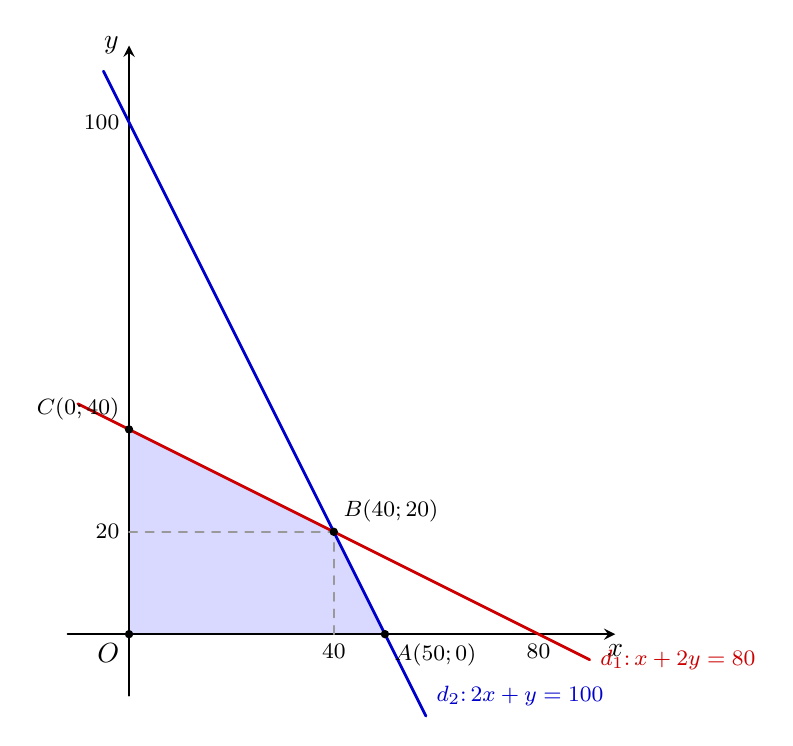
\begin{tikzpicture}[>=stealth, scale=0.065, line join=round, line cap=round]
				% Tô màu miền nghiệm tứ giác OABC
				\fill[blue!15] (0,0) -- (50,0) -- (40,20) -- (0,40) -- cycle;
				
				% Trục tọa độ
				\draw[->, line width=0.8pt] (-12,0) -- (95,0) node[below] {$x$};
				\draw[->, line width=0.8pt] (0,-12) -- (0,115) node[left] {$y$};
				\node[below left] at (0,0) {$O$};
				
				% Đường thẳng d1: x + 2y = 80 => đi qua (80,0) và (0,40)
				\draw[line width=1pt, red!80!black] (-10,45) -- (90,-5) node[right, font=\footnotesize] {$d_1\colon x + 2y = 80$};
				
				% Đường thẳng d2: 2x + y = 100 => đi qua (50,0) và (0,100)
				\draw[line width=1pt, blue!80!black] (-5,110) -- (58,-16) node[above right, font=\footnotesize] {$d_2\colon 2x + y = 100$};
				
				% Đường gióng từ B(40; 20)
				\draw[dashed, line width=0.6pt, gray!80] (40,0) -- (40,20) -- (0,20);
				
				% Điểm đặc biệt và nhãn
				\filldraw[black] (0,0) circle (20pt);
				\filldraw[black] (50,0) circle (20pt) node[below right, font=\footnotesize] {$A(50;0)$};
				\filldraw[black] (40,20) circle (20pt) node[above right, font=\footnotesize] {$B(40;20)$};
				\filldraw[black] (0,40) circle (20pt) node[above left, font=\footnotesize] {$C(0;40)$};
				
				% Các vạch số trên trục
				\node[below, font=\footnotesize] at (40,0) {$40$};
				\node[below, font=\footnotesize] at (80,0) {$80$};
				\node[left, font=\footnotesize] at (0,20) {$20$};
				\node[left, font=\footnotesize] at (0,100) {$100$};
			\end{tikzpicture}
		\end{center}
		Tổng lợi nhuận thu được trong tuần là biểu thức:
		$$F(x; y) = 40x + 50y\text{ (nghìn đồng)}.$$
		Miền nghiệm của hệ bất phương trình là miền tứ giác $OABC$ (kể cả biên) với các đỉnh:
		\begin{itemize}
			\item $O(0; 0)$;
			\item $A(50; 0)$ là giao điểm của đường thẳng $2x + y = 100$ với trục hoành;
			\item $B(40; 20)$ là giao điểm của hai đường thẳng $x + 2y = 80$ và $2x + y = 100$;
			\item $C(0; 40)$ là giao điểm của đường thẳng $x + 2y = 80$ với trục tung.
		\end{itemize}
		Tính giá trị của hàm mục tiêu $F(x; y)$ tại các đỉnh của miền nghiệm:
		\begin{itemize}
			\item Tại $O(0; 0)\colon F(0; 0) = 40 \cdot 0 + 50 \cdot 0 = 0$ (nghìn đồng).
			\item Tại $A(50; 0)\colon F(50; 0) = 40 \cdot 50 + 50 \cdot 0 = 2\,000$ (nghìn đồng).
			\item Tại $B(40; 20)\colon F(40; 20) = 40 \cdot 40 + 50 \cdot 20 = 1\,600 + 1\,000 = 2\,600$ (nghìn đồng).
			\item Tại $C(0; 40)\colon F(0; 40) = 40 \cdot 0 + 50 \cdot 40 = 2\,000$ (nghìn đồng).
		\end{itemize}
		So sánh các giá trị trên, ta thấy $F(x; y)$ đạt giá trị lớn nhất bằng $2\,600$ nghìn đồng tại $(x; y) = (40; 20)$.\\
		Vậy cơ sở cần may $40$ chiếc túi loại $A$ và $20$ chiếc túi loại $B$ để tổng lợi nhuận thu được là lớn nhất ($2\,600\,000$ đồng).
	}
\end{ex}

% --- CÂU 5 ---
\begin{ex}
	Một cột tháp phát sóng truyền hình có chân tháp $H$ và đỉnh tháp $T$ dựng vuông góc với mặt đất nằm ngang. Hai vị trí quan sát $A$ và $B$ trên mặt đất nằm về cùng một phía so với chân tháp sao cho ba điểm $A, B, H$ thẳng hàng và khoảng cách $AB = 45\text{ m}$. Từ các vị trí $A$ và $B$, người ta đo được góc nâng nhìn lên đỉnh tháp lần lượt là $\widehat{TAH} = 30^\circ$ và $\widehat{TBH} = 45^\circ$. Bỏ qua chiều cao của thiết bị đo. Tính chiều cao $HT$ của cột tháp (làm tròn kết quả đến hàng phần mười của mét).
	\begin{center}
		\begin{tikzpicture}[line join=round, line cap=round, scale=0.9]
			% Mặt đất
			\draw[line width=1pt] (-1,0) -- (8,0) node[below] {Mặt đất};
			
			% Tọa độ các điểm: H = (6,0), T = (6, 3.69), B = (2.31, 0), A = (-0.5, 0)
			\coordinate (H) at (6,0);
			\coordinate (T) at (6,3.5);
			\coordinate (B) at (2.5,0);
			\coordinate (A) at (-0.5,0);
			
			% Tháp HT
			\draw[line width=2pt, red!80!black] (H) -- (T) node[above] {$T$};
			\draw (H) rectangle ++(-0.25,0.25); % Kí hiệu góc vuông tại H
			
			% Các tia ngắm
			\draw[line width=1pt, blue] (A) -- (T);
			\draw[line width=1pt, blue] (B) -- (T);
			
			% Điểm và nhãn
			\filldraw[black] (A) circle (1.5pt) node[below] {$A$};
			\filldraw[black] (B) circle (1.5pt) node[below] {$B$};
			\filldraw[black] (H) circle (1.5pt) node[below] {$H$};
			
			% Đoạn AB
			\draw[<->, dashed] ([yshift=-12pt]A) -- ([yshift=-12pt]B) node[midway, fill=white, font=\footnotesize] {$45\text{ m}$};
			
			% Cung tròn góc
			\draw (0.5,0) arc (0:30:1);
			\node at (0.9,0.3) {\footnotesize $30^\circ$};
			
			\draw (3.3,0) arc (0:45:0.8);
			\node at (3.6,0.35) {\footnotesize $45^\circ$};
		\end{tikzpicture}
	\end{center}
	\loigiai{
		Trong tam giác $ABT$, góc $\widehat{TBH}$ là góc ngoài tại đỉnh $B$ nên:
		$$\widehat{ATB} = \widehat{TBH} - \widehat{TAB} = 45^\circ - 30^\circ = 15^\circ.$$
		Áp dụng định lí sin trong tam giác $ABT$, ta có:
		$$\dfrac{BT}{\sin\widehat{TAB}} = \dfrac{AB}{\sin\widehat{ATB}} \implies BT = \dfrac{AB \cdot \sin 30^\circ}{\sin 15^\circ} = \dfrac{45 \cdot 0{,}5}{\sin 15^\circ} \approx 86{,}93\text{ (m)}.$$
		Tam giác $BHT$ vuông tại $H$ có $\widehat{TBH} = 45^\circ$ nên:
		$$HT = BT \cdot \sin\widehat{TBH} = BT \cdot \sin 45^\circ \approx 86{,}93 \cdot \dfrac{\sqrt{2}}{2} \approx 61{,}5\text{ (m)}.$$
		\textit{Cách khác:} Vì tam giác $BHT$ vuông tại $H$ và có $\widehat{TBH} = 45^\circ$ nên tam giác $BHT$ vuông cân tại $H$, suy ra $BH = HT = h$.\\
		Trong tam giác vuông $AHT$ vuông tại $H$:
		$$\tan\widehat{TAH} = \dfrac{HT}{AH} \iff \tan 30^\circ = \dfrac{h}{45 + h} \iff \dfrac{1}{\sqrt{3}} = \dfrac{h}{45 + h}$$
		$$\iff 45 + h = \sqrt{3}h \iff h(\sqrt{3} - 1) = 45 \iff h = \dfrac{45}{\sqrt{3} - 1} \approx 61{,}5\text{ (m)}.$$
		Vậy chiều cao của cột tháp xấp xỉ $61{,}5\text{ m}$.
	}
\end{ex}
